\documentclass[acmtog, authorversion]{acmart}

\usepackage{booktabs} % For formal tables

\usepackage[ruled]{algorithm2e} % For algorithms
\renewcommand{\algorithmcfname}{ALGORITHM}
\SetAlFnt{\small}
\SetAlCapFnt{\small}
\SetAlCapNameFnt{\small}
\SetAlCapHSkip{0pt}
\IncMargin{-\parindent}

% Metadata Information
% \acmJournal{TOG}
% \acmVolume{9}
% \acmNumber{4}
% \acmArticle{39}
% \acmYear{2010}
% \acmMonth{3}

% Copyright
%\setcopyright{acmcopyright}
%\setcopyright{acmlicensed}
%\setcopyright{rightsretained}
%\setcopyright{usgov}
\setcopyright{usgovmixed}
%\setcopyright{cagov}
%\setcopyright{cagovmixed}

% DOI
% \acmDOI{0000001.0000001_2}

% Paper history
% \received{February 2007}
% \received{March 2009}
% \received[final version]{June 2009}
% \received[accepted]{July 2009}


% Document starts
\begin{document}
% Title portion
\title{TBD}
\author{Mengying Sun}
\orcid{1234-5678-9012-3456}
\affiliation{%
  \institution{Michigan State University}
  \department{Department of Computer Science and Engineering}
  \streetaddress{104 Jamestown Rd}
  \city{East Lansing}
  \state{MI}
  \postcode{00000}
  \country{USA}}
\author{Xiaoran Tong}
\affiliation{%
  \institution{Michigan State University}
  \department{Department of Epidemiology and Biostatistics}
  \streetaddress{909 Fee Rd}
  \city{East Lansing}
  \state{MI}
  \postcode{48824}
  \country{USA}
}

\renewcommand\shortauthors{Zhou, G. et al}

\begin{abstract}
  Through this project we seek to predict complex human phenotypes from high dimensional whole genome profiles. To solve the curse of dimensionality, we adopted a two tier modeling by first choosing representative features from chromosome LD blocks, then build a higher tier predictive model upon the first tier output. We expect improvement of predictive accuracy over existing GWAS or kernel based models.
\end{abstract}


%
% The code below should be generated by the tool at
% http://dl.acm.org/ccs.cfm
% Please copy and paste the code instead of the example below. 
%
% \begin{CCSXML}
% <ccs2012>
%  <concept>
%   <concept_id>10010520.10010553.10010562</concept_id>
%   <concept_desc>Computer systems organization~Embedded systems</concept_desc>
%   <concept_significance>500</concept_significance>
%  </concept>
%  <concept>
%   <concept_id>10010520.10010575.10010755</concept_id>
%   <concept_desc>Computer systems organization~Redundancy</concept_desc>
%   <concept_significance>300</concept_significance>
%  </concept>
%  <concept>
%   <concept_id>10010520.10010553.10010554</concept_id>
%   <concept_desc>Computer systems organization~Robotics</concept_desc>
%   <concept_significance>100</concept_significance>
%  </concept>
%  <concept>
%   <concept_id>10003033.10003083.10003095</concept_id>
%   <concept_desc>Networks~Network reliability</concept_desc>
%   <concept_significance>100</concept_significance>
%  </concept>
% </ccs2012>  
% \end{CCSXML}

% \ccsdesc[500]{Computer systems organization~Embedded systems}
% \ccsdesc[300]{Computer systems organization~Redundancy}
% \ccsdesc{Computer systems organization~Robotics}
% \ccsdesc[100]{Networks~Network reliability}

%
% End generated code
%

% We no longer use \terms command
\terms{AI, Algorithms, Performance}

\keywords{ReLU}


\thanks{This work is supported by the National Science Foundation,
  under grant CNS-0435060, grant CCR-0325197 and grant EN-CS-0329609.

  Author's addresses: G. Zhou, Computer Science Department, College of
  William and Mary; Y. Wu {and} J. A. Stankovic, Computer Science
  Department, University of Virginia; T. Yan, Eaton Innovation Center;
  T. He, Computer Science Department, University of Minnesota; C.
  Huang, Google; T. F. Abdelzaher, (Current address) NASA Ames
  Research Center, Moffett Field, California 94035.}


\maketitle


\section{Introduction}
The current prediction of complex phenotypes from whole genome profile is far from satisfactory, leaving large gap between heritability estimated by classical family study and the those explained by current genetic predition methods using large number of genomic variants. Unlike the thoroughly studied question domains such as imaging, acoustic, and texture language, owning to the innovation of artificial intelligence, in particular the deep learning, genetics based prediction suffers obvious difficulty due to the sheer size of individual profiles. A genomic profile could easily reach an order of hundreds of thousands variables thanks to the contemporary genotyping pipelines. The desire of more accurately predict phenotypes motivate approaches that exhausts all available information, yet the size of profile rended most solutions computationally intractable. An obverious work around is variable selection, such as dropping all rare mutation sites that comprises 90\% of the genome, a technique widely practiced by many genome-wide association studies (GWAS) through out the last decade, despite the aforementioned low explanatory power over expected heritibility[]. The first G-matrix propagated kernel based methods into the field of genetics which is capable of taking the entire genome variables under reasonable time to build a predictive model, but these models are still under-performed when faced with phenotypes of mediocre heritibility (i.e. the empirical estimate from pedigree or twin studies).

Despite the horrendous size of the genomic profile, it is well known that genomic variables that are closely located in a section of a chromosome are highly correlated due to the mutual attraction between neighboring nucleotides in the double helix molecules - a phenomenon called linkage disequilibrium (LD). More formally, LD states that the frequency of observing a particular type of variation at one site is not independent to the joint configuration observed at some other sites, and such non-independence grow stronger with increasing proximity of sites in question. As a result, there is a nature division of the genome into several thousands to tens of thousands of LD blocks, such that the variables within a block are significantly more correlated than those between blocks. If we assume each LD block can be represented by a small number of selected variables, or by low dimensional features, given that they are highly correlated, the complexity of the orignal modeling problem can be reduced from the order of hundreds of thousands to tens of thousands or even less.

Another characteristic of the genome worth reiteration is that the bulk of variables represent rare or extremely rare mutations in the population, that is, only a handful of individuals has non-zero values in virtually 90\% of the variables. Such extreme sparsity justifies the strong motivation of variable selection, for example, by quickly screening all variables with simple linear regression against the phenotype of interests, followed by discarding those failed to pass a significance threshold, which indeed is a fairly common practice of GWA up till today. It is debatable however, from a biological and genetic perspective, that rare variations can still be moderately powerful and should not be discarded simply because there is inadequate samples to demonstrate their effect [].

In this study we aim to predict the standard phenotype - body height, using variable through out the entire genome. The general approach is to first divide the profile into LD blocks, after which either select a small subset or extract low dimensional features from each block (tire 1), and later learn the predictive model from the selected or extracted variables (tire 2). The identification of LD blocks is supported by popular genetic analysis tools. For each block, the variables can be selection via linear regression with information criteria (e.g., AIC and BIC), which is rather fast, or, one could build a stacked autoencoder to extract a few high-order features, which is slower but can better preserve information of all variables. For the tier 2 modeling, a neural network or high dimensional linear regression can be of choic.

Regarding the training of neural networks, either for the lower tier feature extraction or higher tier prediction modeling, the norm taken from machine learning apparatus is the pursuit of deeper networks, a trend started by revival of multi-layer sigmoid network through pre-training \cite{DL:Intro1}, and pushed to a new depth by rectified linear unit (ReLU) \cite{DL:Relu1}, which indeed scored many victories in the last decade\cite{DL:Intro2, DL:Intro3}. However, aside from computation and storage, going deep is not without a cost. The network tends to overfit and stagnate, even if Relu is promoting both mobility and sparcity via constant gradient on positive input and zero gradient on negative input, respectively. The recent development has been mainly topological enhancement, such as random dropout of neurons to encourage heterogeneous feature capture \cite{DL:DRP1}, short circuiting layers via residual learning to improve gradient flow\cite{DL:DRL1}, companion trainers to promote uniform evolution of the network, and the conglomeration of topological tweaks via implict ensemble \cite{DL:SWP1}. Nonetheless, they all stress the central doctrine that ``deeper is better'', which may not be the case when the domain shifts from visual, acoustic and texture to genomics, considering it innate sparse and binary nature, which also lacks obvious high order features (e.g., what is the analogy of facial features in terms of genome?). We shall decide the type of network suitable to work with genomic profiles through large number of benchmarks on randomly selected genome sites.

\section{Material and Method}
The body height target variable and corresponding whole genome profiles were obtained from UK Biobank [?], a prospective cohort study of over 500K individuals from across the United Kingdom during 2006 and 2010. In our study, the geomic variables are exclusively single nucleotide polymorphisms (SNPs). A total of 589,028 SNP readings for 102,110 individuals passed the following quality control: (i) removal of SNPs with MAF (minor allel frequency) < 0.05, that is, genome sites of rare variation; (ii) removal of SNPs with missing values in more than 30\% of the participants; (iii) removal of individuals with incomplete mapping between phenotype and genotype profiles. To evaluate generalization performance, we split data into training and testing set, with 80,000 observations for training and 22,110 for testing. 

We identify LD blocks using the third party tool PLINK[?], which produces subsets of markers that are in approximate linkage disequilibrium (LD) with each other. It is based on correlations between genotype allele counts. Two variants are normally considered to be in strong LD if the bottom of the 90\% D-prime confidence interval is greater than 0.70, and the top of the confidence interval is at least 0.98. Moreover, only pairs of variants within 200 kilobases of each other are considered.  A total number of 190,174 blocks were identified using these criteria.

To facilitate LD block autoencoder training, the genomic variables are flattened by lining up the two copies of nucleotides taken from a pair of homogeneous chromosomes, which ends up with a binary vector taking value 0 as no variation, and 1 as varying from the human reference genome [?].

After variable selection, we will construct learning models for predicting height using selected markers. Two different approaches are considered: (i) Bayesian generalized linear regression; (ii) Neural Networks. Prediction accuracy is measured by correlation between predicted height and true height in testing procedure. 

\subsection{Genome-wide association Study (GWAS)}
A genome-wide association study (GWAS) was performed for training data set. 

\begin{figure}[h]
  \centering
  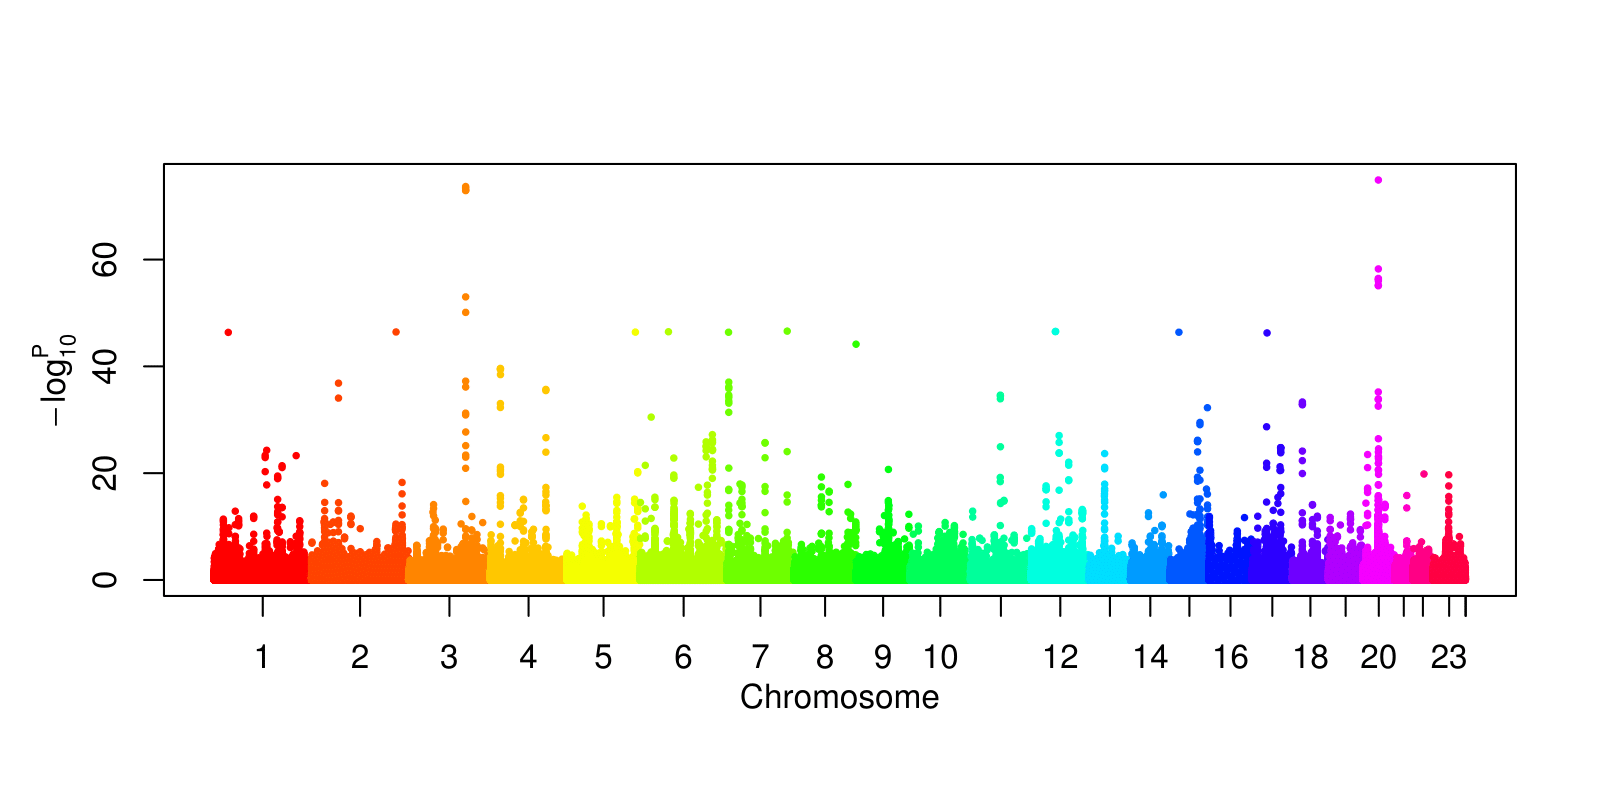
\includegraphics[width=3.5 in, trim=0 0 0in 0]{img/gwas_height}
  \caption{Negative log p-value for 600K markers.}
  \label{gwas}
\end{figure}

\subsection{Variable Selection within LD Block}
To achieve genomic variable selection, first we perform a traditional GWAS screening of the training data set, by which, the target variable - body height, is linearly regressed on each genomic variable (i.e. a SNP) one at a time, and the p-value of the regression coeficient is recorded. By plotting all 600K p-values in the negative log(10) scale (Figure \ref{gwas}), the classical GWAS is near completion by picking out variables with negative log p-values above a pre-defined threshold (usually 8 [?]) that signifies strong association between the said variable and phenotype of interest. Here, we seek to select variable not based on a universal cut off but rather on a block by block bases.

For each LD block, variable selection is done via four different approaches: (i) top-k selection, in which we ordered adjusted p-values descendingly in a global sense and select top k markers across whole genome; (ii) block-top-k selection, in which we selected top-k markers based on adjusted p-value within each block; (iii) stepwise selection based on information criteria, in which we use AIC and BIC to select markers within each block; (iv) selection based on LASSO in each block. Summary for selections are shown in Figure \ref{fig:AIC} and Figure {\ref{fig:BIC}}. For AIC, we end up with 123,393 selected SNPs in 80,813 blocks, while for BIC we got 6022 selected SNPs in 5554 blocks. BIC penalizes feature size more strongly than AIC and therefore tends to favor less selected markers. 

\begin{figure}[!h]
  \centering
  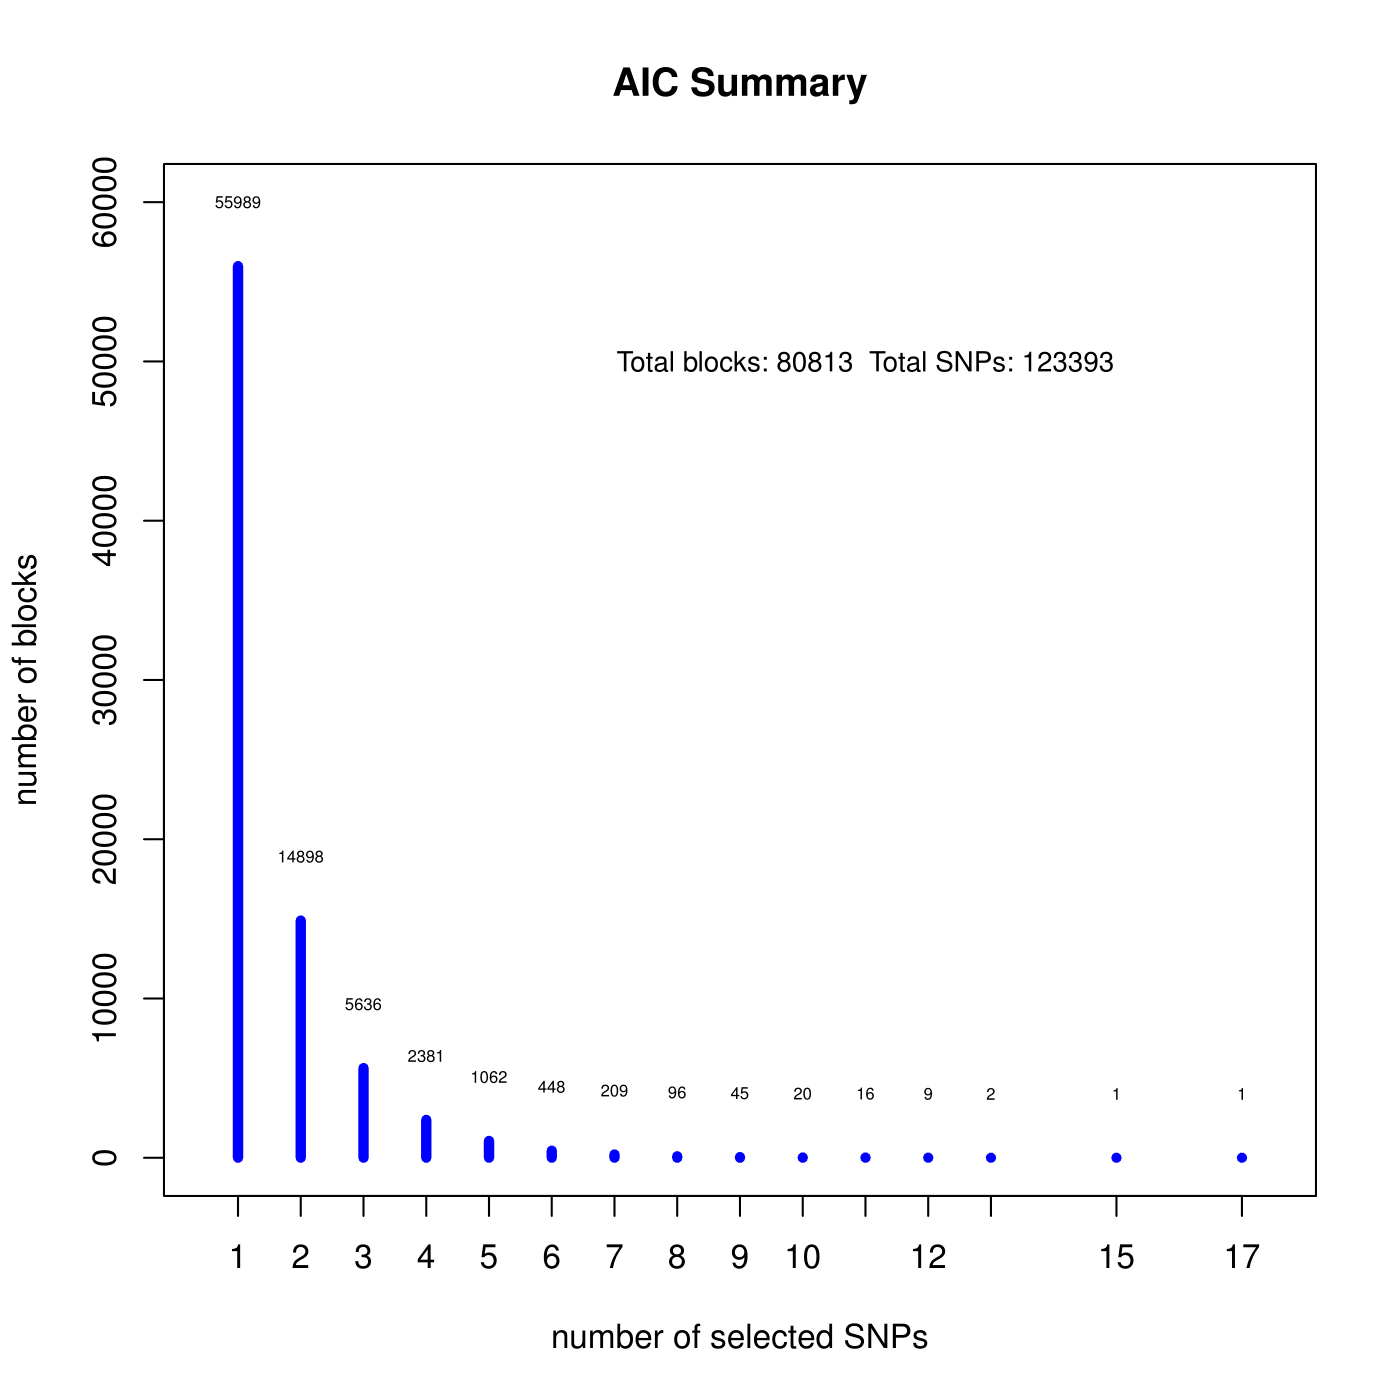
\includegraphics[width=3.5 in, trim=0 0 0in 0]{img/AIC_summary}
  \caption{Variable selection by AIC}
  \label{fig:AIC}
\end{figure}
\begin{figure}[!h]
  \centering
  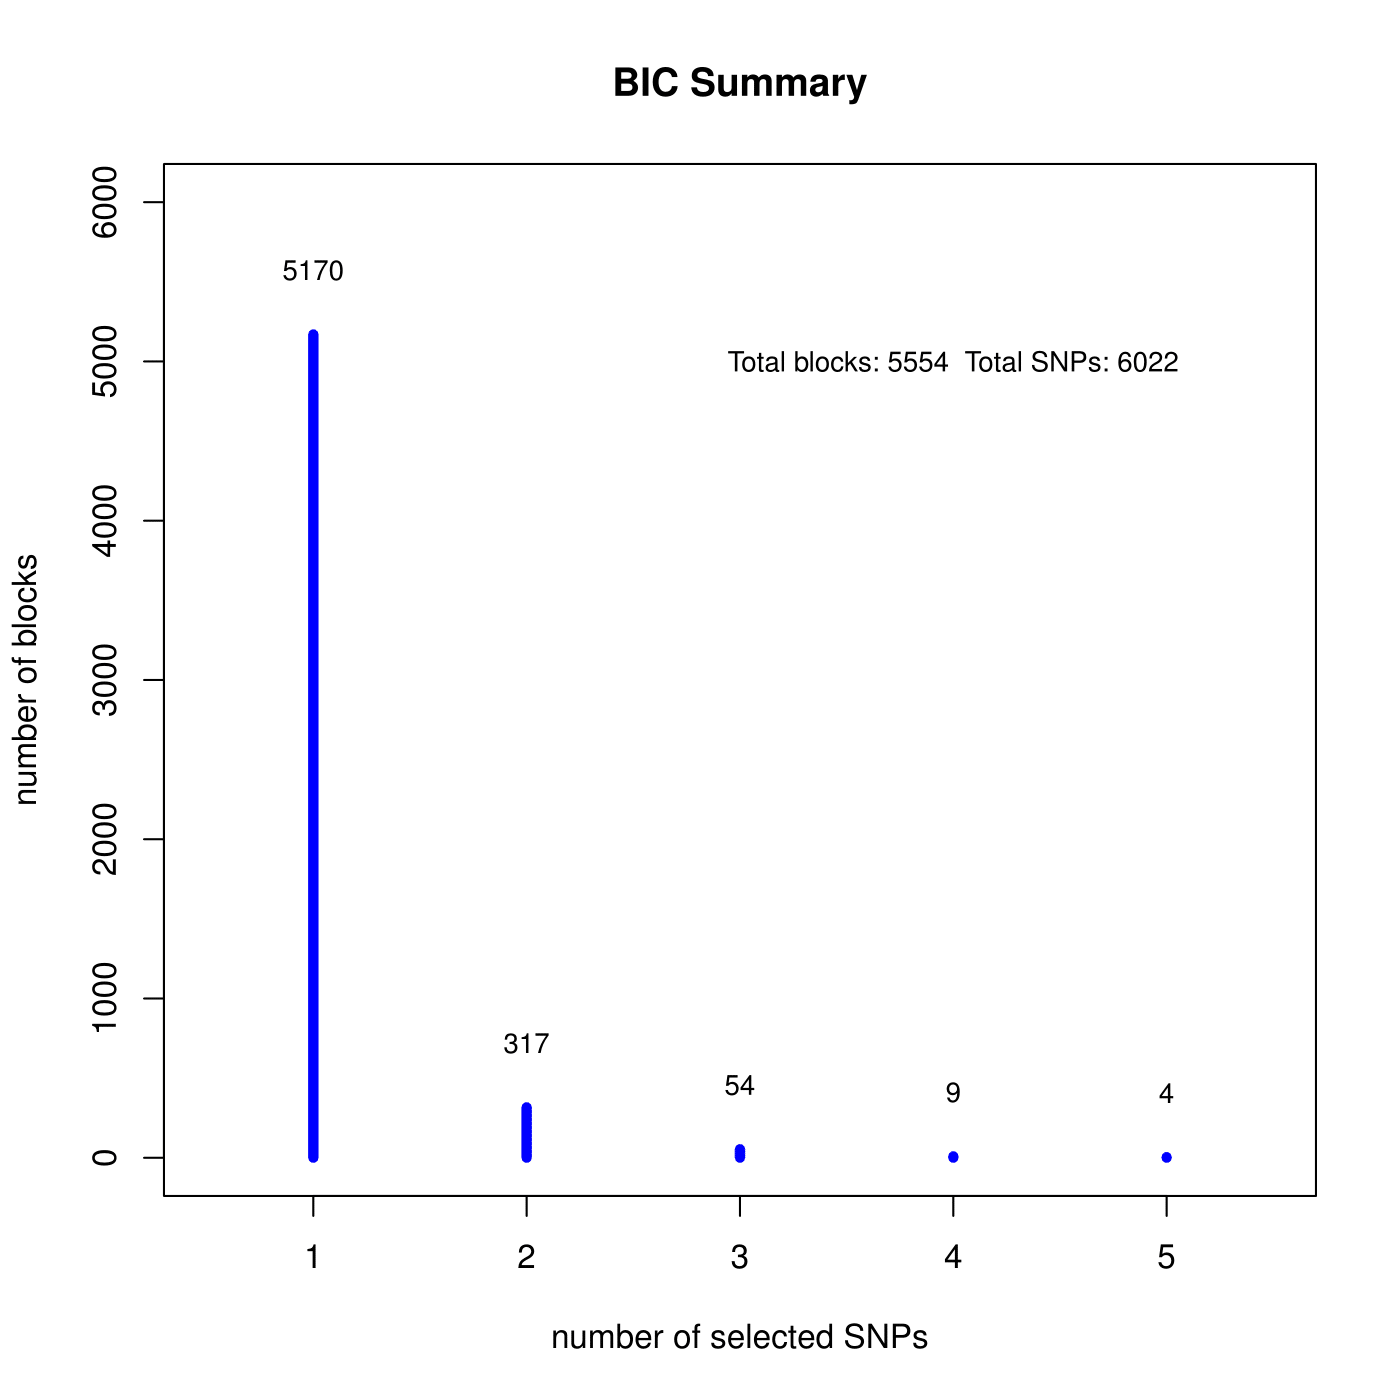
\includegraphics[width=3.5 in, trim=0 0 0in 0]{img/BIC_summary}
  \caption{Variable selection by BIC}
  \label{fig:BIC}
\end{figure}


\subsection{Variable Extraction within LD Block}
We first assess the performance of sigmoid and relu autoencoders on randomly chosen genome segments of $2^9 = 512$ consecutive variables ($1024$ after flattening homogeneous chromosome), which is intended to find out network better tuned for genomic related tasks. The benchmarks do not use the target body height data, but instead rely on 2502 participants of ``1000 genome'' project hosted on National Center for Biotechnology Information (NCBI), doing so ensure the performance of genomic autoencoders be independent of the target data. The overall performance is gauged by convergence rate and the ability to lower the reconstruction error on one fifth of the data hold out from training.

The initiall setting halve the data dimension with every additional encoder layer, until the output code have only one dimension, which gives $1024, 512, \dots, 2, 1$ nodes for a total of 10 encoder layers. Both sigmoid and relu activation are tested. For the relu case, the last reconstruction layer also use sigmoid function in order to match the binary genomic variables. Convergence is declared when testing error on the hold out data constantly rises for the last 50 epochs, and a total budget of 1000 epochs are reserved for each benchmark trial should it fail to converge. The mean performance of 1000 trails is shown in Figure (\ref{fig:ae0}), for trails converged before reaching 1000 epoch, errors for the remaining epochs are extrapolated from the laster one right before the stop.
\begin{figure}[h]
  \centering
  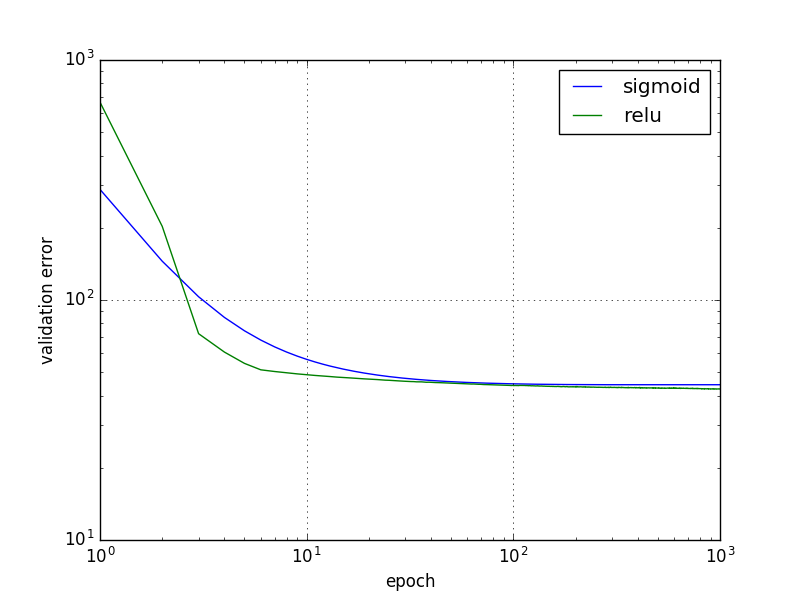
\includegraphics[width=0.35\textwidth]{img/00}
  \caption{Autoencoder Test, depth=10}
  \label{fig:ae0}
\end{figure}
Under the the initial setting, relu based networks maintained a small edge over sigmoid networks after long training in terms of testing error, and also significantly faster to reach convergence.

The subsequent tests reduce encoding depth from 10 to 9 and 8, so the relative improvement of information preservation can be observed when the encoding ratios become less demanding. The mean performance of 1000 trails is shown in Figure (\ref{fig:ae1}) and (\ref{fig:ae2}).
\begin{figure}[h]
  \centering
  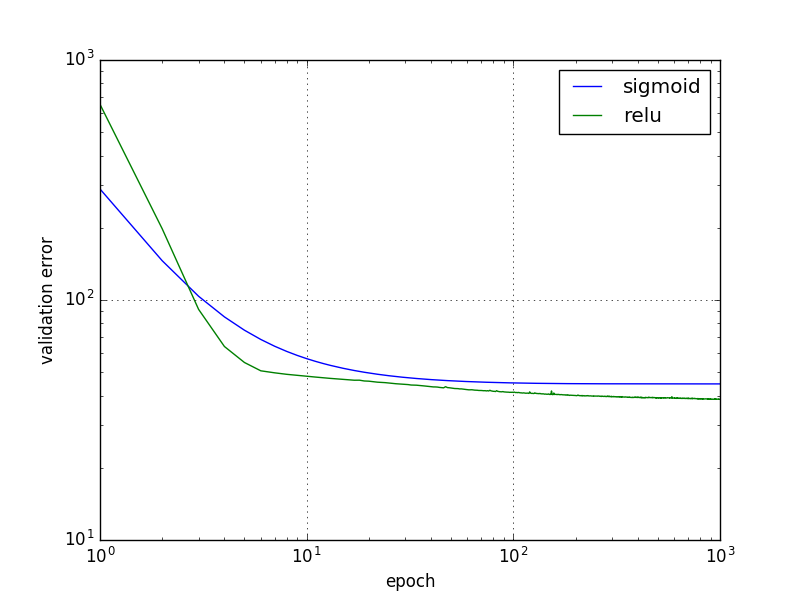
\includegraphics[width=0.35\textwidth]{img/01}
  \caption{Autoencoder Test, depth=9}
  \label{fig:ae1}
\end{figure}
\begin{figure}[h]
  \centering
  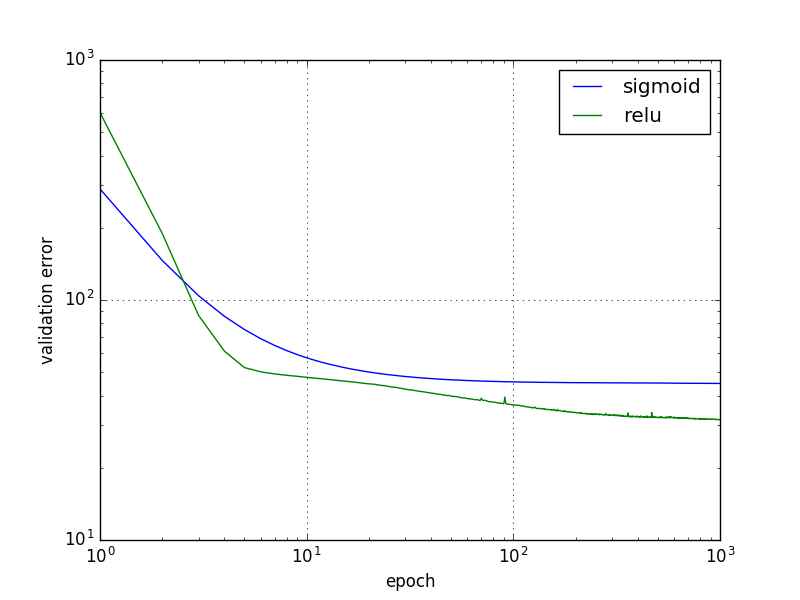
\includegraphics[width=0.35\textwidth]{img/02}
  \caption{Autoencoder Test, depth=8}
  \label{fig:ae2}
\end{figure}

We see the redu network gained more performance than that of sigmoid network when encoding depth is reduced. We did not further optimize the sigmoid network by greedy layer-wise pre-training, not only because it gives the sigmoid unfair edges, but also means more time consuming when dealing with 10 thousand LD blocks. Overall, it seems that relu is better suited to process discrate and highly spare genomic data.
<Another test that doulbes the network depth is also on the way, in order to see if deep structure helps to maintain information while fixing encoder output size, though the first few attemp failed due to dramatically increased training expenditure.>

\section{Up comming work}
If a massive number of autoencoder is affordable, we would try out the mass tier 1 autoencoder + tier 2 networks approach, alongeside with tier 1 linear variable selection (guided by AIC or BIC) + tier 2 networks approach. If the the tier 2 network become unafforable should the post-screening number of LD blocks is rather huge, we will adopt the aforementioned Bayesian Generalized Linear Regression at least.
<By reducing the number of trial and per trial budget, assess possible improvement of genomic feature extraction when autoencoders goes deeper.>
<From the the current variable selection trails, the BIC based approach seems to be more supportive to a higher tier neural network, since the number of variables passing the criteria is small - 6K.>

% Bibliography
\bibliographystyle{ACM-Reference-Format}
\bibliography{ref}

\end{document}
